\chapter{Introducción}
\label{cap:introduccion}
\setcounter{page}{1}

El avance tecnológico constante ha transformado nuestra forma de percibir el mundo. Tecnologías como la robótica han dado lugar a dispositivos capaces de realizar tareas que antes parecían imposibles. Hace medio siglo, la idea de un aparato que pudiera barrer de manera eficiente o de un vehículo que se condujera solo era pura fantasía. Hoy, los vehículos inteligentes han pasado de ser un concepto de ciencia ficción a convertirse en una realidad que está revolucionando el transporte y remodelando nuestras ciudades.

La capacidad de los vehículos autónomos para desenvolverse de manera segura en entornos complejos, no solo reducen los errores humanos, sino que también abren nuevas oportunidades en ámbitos esenciales. Desde mejorar la seguridad vial y promover la eficiencia energética hasta fomentar la inclusión social, convirtiéndose en pilares fundamentales para el desarrollo de ciudades más sostenibles. Aunque todavía queda un largo camino por recorrer, estos avances permiten vislumbrar un futuro donde el tráfico sea más fluido, los recursos urbanos estén mejor aprovechados y las personas con movilidad reducida o dificultades para conducir tengan un acceso más equitativo a los servicios de transporte.

En este \ac{TFG}, nos centraremos en los sistemas de conducción autónoma, explorando su aplicación en la movilidad inteligente dentro de entornos urbanos. Analizaremos cómo la \ac{IA} y \ac{ML} contribuye a este campo, tanto en el aspecto sensorial como en el de control. En el ámbito del control, nos enfocaremos en \ac{DRL}, evaluando diferentes algoritmos para determinar cuáles ofrecen los mejores resultados.

\section{Vehículos autónomos}
\label{sec:vehículos}

Un vehículo autónomo es aquel capaz de realizar todas las funciones de conducción entre un origen y un destino sin la intervención de un ser humano, más allá de indicar el punto de inicio y final del trayecto. En los niveles intermedios, donde aún se requiere la actuación de un conductor, la autonomía no es total.

En la actualidad, la industria automotriz ha desarrollado una amplia gama de \ac{ADAS}, cuyo objetivo principal es reducir el riesgo de accidentes. Estos sistemas utilizan una red de sensores para analizar el entorno de conducción, procesando la información mediante la electrónica del vehículo. Con esta información, el sistema toma decisiones predefinidas y puede intervenir en elementos como el acelerador, los frenos o la dirección. Entre sus funcionalidades más comunes hoy en día se incluyen aquellas que corrigen desvíos involuntarios del carril o alertan al conductor sobre peligros inminentes que requieren una respuesta inmediata. Aunque estos avances representan pasos intermedios hacia la conducción autónoma completa, los \ac{ADAS} continúan asistiendo al conductor en tareas específicas, aún requieren su supervisión activa. Los \ac{ADAS} establecen las bases para la implementación futura de sistemas totalmente autónomos.

La Sociedad de Ingenieros Automotrices (\ac{SAE}) ha establecido una clasificación estandarizada de los niveles de autonomía de los vehículos, que abarca desde la conducción completamente manual hasta la conducción completamente autónoma. Esta categorización divide los vehículos autónomos en seis niveles, según el grado de intervención que se requiere del conductor y la capacidad del sistema del vehículo para tomar control \cite{autobild-autonomous}.

\begin{figure} [ht]
  \begin{center}
    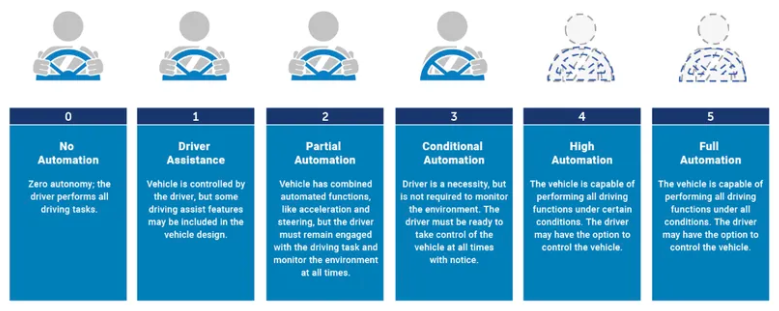
\includegraphics[width=13cm]{figs/introducción/niveles.png}
  \end{center}
  \caption{Niveles de autonomía explicados(\ac{SAE}).}
  \label{aut-levels}
  \end{figure}

\begin{itemize}
    \item \textit{Nivel 0:} Ninguna autonomía. El conductor es completamente responsable de todas las tareas de conducción.
    \item \textit{Nivel 1:} Asistencia al conductor. El vehículo puede realizar una función específica (como el control de crucero), pero siempre requiere la supervisión activa del conductor.
    \item \textit{Nivel 2:} Automatización parcial. El vehículo cuenta con sistemas que pueden replicar tareas de conducción, pero el conductor debe estar preparado para intervenir en cualquier momento.
    \item \textit{Nivel 3:} Automatización condicional. El vehículo puede tomar control completo en determinadas condiciones, pero el conductor debe estar disponible para retomar el control si el sistema lo solicita.
    \item \textit{Nivel 4:} Alta automatización. El vehículo puede operar de forma autónoma en condiciones específicas, sin necesidad de intervención humana, aunque pueden existir limitaciones geográficas o contextuales.
    \item \textit{Nivel 5:} Automatización total. El vehículo es completamente autónomo y no requiere intervención humana en ningún momento ni bajo ninguna circunstancia.
\end{itemize}

Hoy en día, no existen vehículos completamente autónomos disponibles comercialmente. Lo más cercano a la autonomía total que se puede encontrar en el mercado es el nivel 2+. Sin embargo, existen numerosos proyectos en desarrollo que están alcanzando el nivel 3, como es posible ver videos promocionales que muestran coches en movimiento sin intervención activa del conductor. No obstante, estas demostraciones se realizan en entornos extremadamente controlados y con condiciones específicas.

En algunos países, la legislación aún no permite el uso de vehículos autónomos de nivel 3 o superior. Por ejemplo, en España, la ley prohíbe que el conductor suelte el volante durante la conducción, lo que impide el uso de vehículos de nivel 3. En cambio, en California, es legal el uso de vehículos con conducción semi-autónoma, lo que permite al conductor levantar las manos del volante en ciertas circunstancias \cite{carwow-autonomous}. 

\subsection{Evolución histórica de los vehículos autónomos}
\label{sec:historia}

La primera vez que se puso en práctica el concepto de vehículo autónomo fue en 1925 en Nueva York. El ingeniero Francis Houdina diseñó el primer coche sin conductor, controlado de forma remota por radiofrecuencia. Sin embargo, este vehículo requería un coche escolta desde el cual se dirigía.

En 1939, el diseñador industrial estadounidense Norman Bel Geddes revolucionó las ideas sobre transporte al presentar, en la Feria Futurama, un concepto visionario: vehículos eléctricos guiados de manera autónoma mediante radiocontrol en carreteras automáticas con circuitos eléctricos integrados en el pavimento. Aunque no se trataba del concepto moderna de coche autónomo, esta propuesta marcó un antes y un después, despertando el interés de numerosas empresas tecnológicas en el campo de la conducción autónoma.

\begin{figure} [ht]
  \begin{center}
    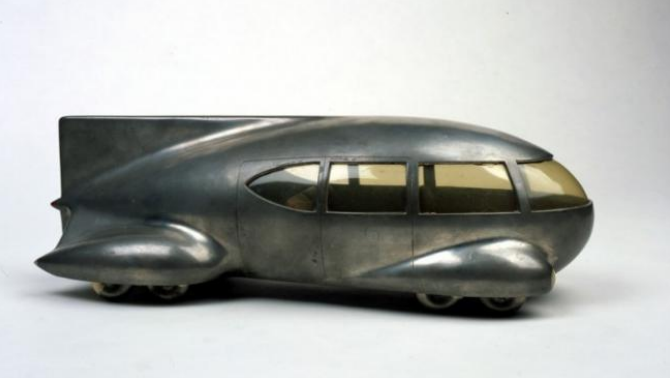
\includegraphics[width=8cm]{figs/introducción/coche_geddes.png}
  \end{center}
  \caption{Coche diseñado por Norman Bel Geddes en 1933.}
  \label{coche-geddes}
  \end{figure}

La mayoría de los avances significativos en este ámbito se deben a Ernst Dickmanns, un profesor alemán experto en \ac{IA}. Dickmanns lideró la creación del primer coche autónomo moderno, combinado la visión sacádica (un movimiento
rápido del ojo, cabeza u otras partes del cuerpo de animales o dispositivos) con cálculos probabilísticos y computación paralela. En 1987, diseñó una furgoneta \textit{Mercedes-Benz} equipada con esta tecnología, logrando conducirla exitosamente por una autopista a velocidades de hasta 100 km/h en condiciones de tráfico controladas. En 1994, lo superó con el modelo  \textit{Mercedes 500 SEL}, conocido como \textit{VaMP}, que recorrió más de 1.000 kilómetros en la carretera de circunvalación de París. Este vehículo alcanzó velocidades de hasta 130 km/h y era capaz de realizar maniobras complejas, como adelantamientos.

\begin{figure}[ht]
  \begin{center}
    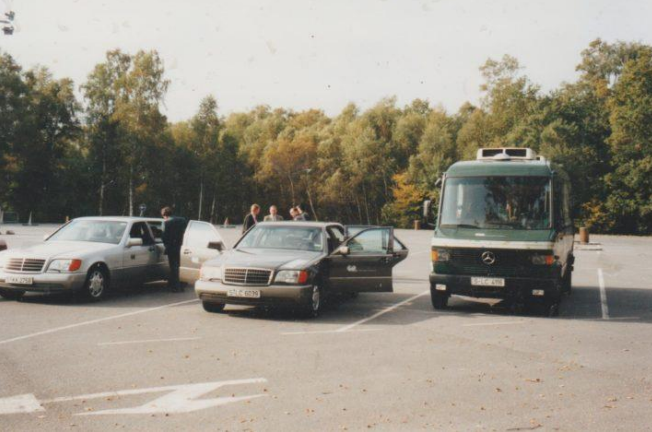
\includegraphics[width=7cm]{figs/introducción/paris_1994.png}
  \end{center}
  \caption{Demostración en vico del funcionamiento de \textit{VaMP} en París.}
  \label{coche-geddes}
\end{figure}

La Comisión Europea, consciente del potencial de los coches autónomos, destinó 800 millones de euros al proyecto  \textit{EUREKA Prometheus}, una iniciativa que marcó un hito en el desarrollo de esta tecnología. Este programa facilitó la creación de numerosos prototipos que sentaron las bases de los vehículos autónomos modernos  \cite{history-vehicles}. Actualmente, este campo es liderado por empresas como \textit{Waymo}, \textit{Tesla}, \textit{Cruise} y \textit{NVIDIA } \cite{ai-self-driving-cars}.

\textit{Waymo} \footnote{\url{https://waymo.com/intl/es/}}, el sistema de conducción autónoma desarrollado por \textit{Google}, se ha consolidado como un referente en el sector de los vehículos sin conductor. Gracias a la integración de \ac{IA}, \textit{Waymo} destaca por su capacidad para planificar rutas complejas y reaccionar de forma inteligente ante diversos escenarios en la carretera. Un vehículo \textit{Waymo} es capaz de operar de manera segura y autónoma siguiendo los siguientes pasos:

\begin{itemize}
    \item El conductor o pasajero establece el destino y el software del vehículo calcula automáticamente la mejor ruta.
    \item Un sensor \ac{LiDAR} giratorio, montado en el techo, escanea un rango de 60 metros alrededor del vehículo, generando un mapa tridimensional dinámico del entorno.
    \item Un sensor ubicado en la rueda trasera izquierda mide los movimientos laterales del vehículo para determinar su posición exacta en relación con el mapa 3D.
    \item Los sistemas de radar, instalados en los parachoques delantero y trasero, calculan la distancia a los obstáculos cercanos.
    \item La inteligencia artificial del vehículo recopila datos de todos los sensores, así como de \textit{Google Street View} y cámaras internas, para interpretar el entorno y tomar decisiones.
    \item La \ac{IA} simula los procesos perceptivos y de toma de decisiones de un ser humano mediante aprendizaje profundo, controlando sistemas clave como los frenos y la dirección.
    \item El software del vehículo consulta \textit{Google Maps} para obtener información anticipada sobre señales de tráfico, puntos de referencia y semáforos.
\end{itemize}

\begin{figure}[ht]
  \begin{center}
    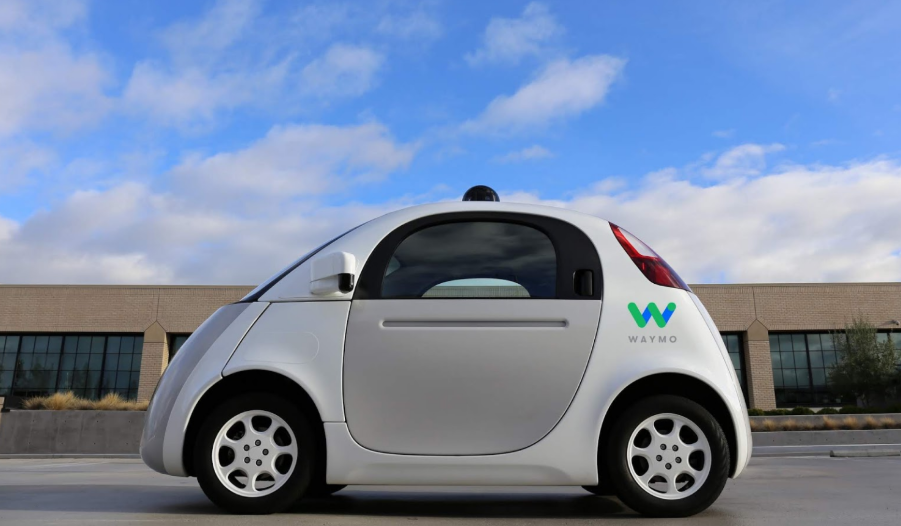
\includegraphics[width=6cm]{figs/introducción/waymo.png}
  \end{center}
  \caption{Coche autónomo de Waymo con sensores y tecnología avanzada.}
  \label{waymo}
\end{figure}

Un claro ejemplo son sus taxis sin conductor \footnote{\url{https://www.youtube.com/watch?v=JHgr9SgeicM}}, los cuales están ganando popularidad en ciertos estados de Estados Unidos, como San Francisco, donde  se han desplegado flotas de vehículos completamente autónomos para transporte de pasajeros. Estos taxis, que no requieren la intervención de un conductor humano, han generado interés por su potencial para revolucionar el transporte urbano, aunque también han suscitado debates sobre su regulación, seguridad y el impacto en el empleo dentro del sector del transporte.

\textit{Tesla} ha logrado un avance notable con su sistema \textit{Autopilot}, capaz de mantener un control preciso utilizando sofisticados algoritmos de \ac{IA} para tomar decisiones rápidas y precisas. Modelos como el \textit{Model 3} y el \textit{Model Y} incorporan el sistema \textit{Tesla Vision}, que prescinde del uso de radar y utiliza un avanzado conjunto de cámaras junto con el procesamiento de redes neuronales desarrolladas por \textit{Tesla}. Este sistema ofrece tres niveles principales: Piloto automático, Piloto automático mejorado y Capacidad de conducción autónoma total.

\subsubsection{Piloto Automático}

\begin{itemize}
    \item \textit{Control de crucero adaptativo al tráfico}: ajusta automáticamente la velocidad del vehículo para adecuarse al flujo del tráfico.
    \item \textit{Autogiro}: permite mantener al vehículo dentro de un carril claramente delimitado.
\end{itemize}

\subsubsection{Piloto Automático Mejorado}

\begin{itemize}
    \item \textit{Cambio automático de carril}: facilita el cambio al carril adyacente cuando el conductor activa el intermitente.
    \item \textit{Navegar en piloto automático (Beta)}: mejora la funcionalidad de cambio de carril automático al proporcionar orientación activa para transitar desde la incorporación hasta la salida de autovías. Incluye sugerencias de cambio de carril y asistencia en intersecciones.
    \item \textit{Autopark}: automatiza el proceso de estacionamiento en paralelo o perpendicular.
    \item \textit{Dumb Summon}: permite mover el vehículo dentro o fuera de plazas de aparcamiento estrechas mediante la aplicación móvil.
    \item \textit{Actually Smart Summon}: mejora las capacidades del vehículo para moverse de manera autónoma en entornos complejos, como plazas de aparcamiento, maniobrando alrededor de obstáculos y localizando al conductor dentro del área cercana.
\end{itemize}

\subsubsection{Capacidad de Conducción Autónoma Total}

\begin{itemize}
    \item \textit{Integración completa}: incluye todas las funcionalidades del Piloto Automático básico y del Piloto Automático Mejorado.
    \item \textit{Control de semáforos y señales de stop (Beta)}: detecta señales de tráfico como semáforos y señales de alto. A medida que el vehículo se acerca, ajusta automáticamente la velocidad y se detiene.
\end{itemize}

A pesar de las mejoras en el rendimiento que proporcionan estas características, no hacen que el coche sea completamente autónomo, requieren un conductor totalmente atento, con las manos en el volante y preparado para tomar el control en cualquier momento \cite{tesla-autopilot}.

\begin{figure}[ht]
  \begin{center}
    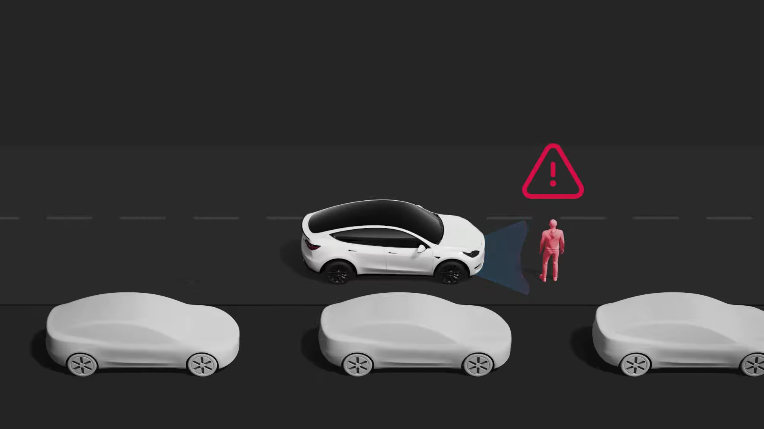
\includegraphics[width=8cm]{figs/introducción/tesla_model_y.png}
  \end{center}
  \caption{\textit{Tesla Model Y} frenando ante un obstáculo.}
  \label{tesla}
\end{figure}

\textit{Cruise}, una empresa de \textit{General Motors}, ha destacado con su vehículo \textit{Cruise AV}, en el que el 40\% de su hardware está diseñado específicamente para la conducción autónoma. Este modelo integra una combinación de cámaras, \ac{LiDAR} y radar, permitiéndole realizar entre 200 y 800 maniobras diarias para sortear vehículos estacionados en doble fila \footnote{\url{https://www.getcruise.com/news/blog/2019/how-self-driving-cars-think-navigating-double-parked-vehicles/?_gl=1*81u4mi*_gcl_au*MTU2MzE4NjQzOC4xNzM2Njg4NzY2s}}. Además, el sistema es capaz de adaptarse a condiciones climáticas adversas, como la lluvia, asegurando una conducción segura y eficiente en entornos urbanos complejos.

\clearpage

\begin{figure}[ht]
  \begin{center}
    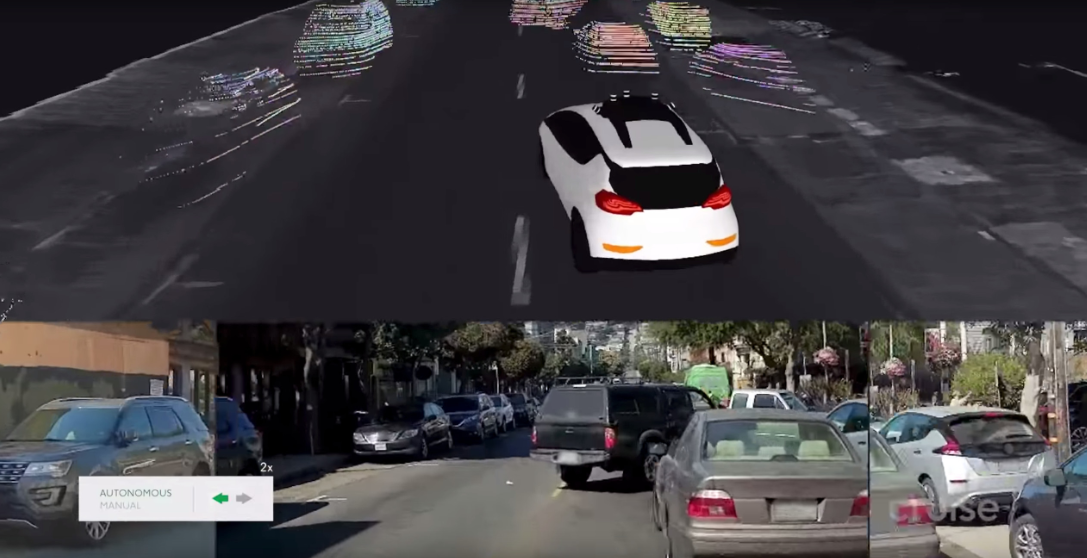
\includegraphics[width=9cm]{figs/introducción/cruise_av.png}
  \end{center}
  \caption{Detección de otros coches del \textit{Cruise AV}.}
  \label{cruise}
\end{figure}

Por último, \textit{NVIDIA} ha desarrollado la plataforma \textit{NVIDIA DRIVE} \footnote{\url{https://www.nvidia.com/es-es/self-driving-cars/?utm_source}}, una solución de computación avanzada que demuestra cómo la inteligencia artificial puede integrarse de manera efectiva en los vehículos autónomos.

\begin{figure}[ht]
  \begin{center}
    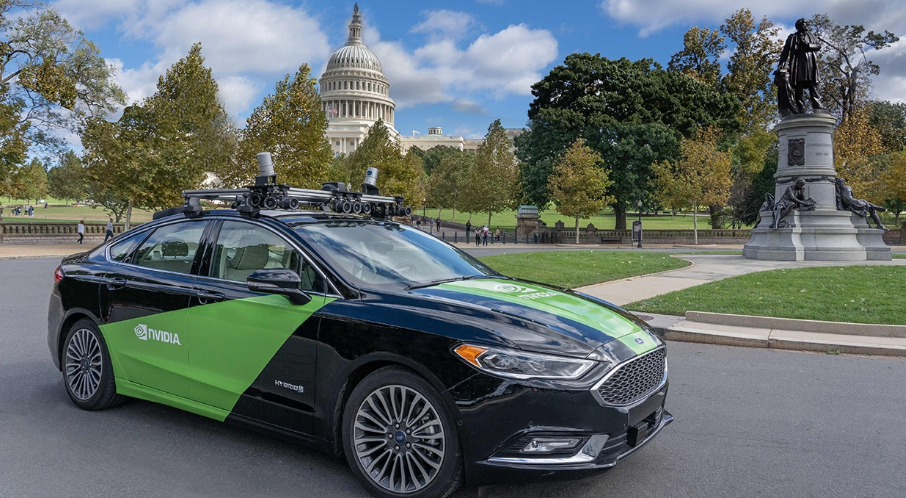
\includegraphics[width=7cm]{figs/introducción/nvidia.png}
  \end{center}
  \caption{Coche autónomo de NVIDIA.}
  \label{nvidia}
\end{figure}

\subsection{Desafíos actuales en la implementación de vehículos autónomos}
\label{sec:desafíos}

Los vehículos autónomos enfrentan numerosos desafíos que deben ser superados para lograr su implementación generalizada. Estos desafíos se dividen principalmente en aspectos técnicos y no técnicos, cada uno con sus propias complejidades que requieren soluciones específicas.

En el ámbito técnico, uno de los mayores retos radica en la detección y análisis de datos. Los vehículos autónomos necesitan identificar obstáculos de manera inequívoca, incluso a altas velocidades y largas distancias. Esto exige un software avanzado capaz de procesar grandes volúmenes de datos en tiempo real con un alto grado de precisión, un área que aún enfrenta importantes limitaciones. Además, garantizar un sistema seguro y fiable implica desarrollar tecnología tolerante a fallos y capaz de operar de manera eficiente en entornos no controlados. En el mundo real, los vehículos autónomos deben enfrentarse a miles de situaciones impredecibles durante la conducción, y los sistemas actuales todavía están lejos de resolver de manera eficiente todas estas incertidumbres.

Otro desafío técnico crucial es la seguridad cibernética. Los vehículos autónomos, especialmente aquellos basados en \ac{DL}, son vulnerables a ataques que podrían comprometer su funcionalidad o la seguridad de sus ocupantes. Por ello, es imprescindible implementar estrategias robustas de defensa para mitigar estos riesgos y generar confianza en la tecnología.

En el ámbito no técnico, las cuestiones legales y éticas presentan una barrera importante. Existe una preocupación creciente sobre la responsabilidad en caso de accidentes, ya que no está claro si la culpa recaería en el fabricante, el desarrollador del software o el propietario del vehículo. También es esencial salvaguardar la privacidad de los datos de los pasajeros, ya que los sistemas autónomos recopilan y procesan grandes cantidades de información personal.

La aceptación por parte de los consumidores y las regulaciones gubernamentales son factores determinantes en el desarrollo de vehículos autónomos. En la actualidad, las políticas y normativas suelen avanzar a un ritmo más lento que el desarrollo tecnológico, lo que complica las pruebas y la implementación a gran escala.

La superación de estos obstáculos requerirá soluciones innovadoras que satisfagan las necesidades de los consumidores, la industria y los gobiernos. La colaboración interdisciplinaria será clave para abordar estos desafíos, sentando las bases de un futuro en el que los vehículos autónomos sean seguros, eficientes y ampliamente aceptados en la sociedad \cite{challenges-autonomous}.

\section{Impacto de la IA en el transporte autónomo}
\label{sec:ia-intro}

Los coches autónomos son sistemas diseñados para tomar decisiones sin intervención humana, procesando flujos de datos provenientes de diversas fuentes a bordo, como cámaras, radares, \ac{LiDAR}, sensores ultrasónicos, unidades \ac{GPS} y sensores inerciales. Estos sistemas utilizan las observaciones recogidas para tomar decisiones sobre la conducción del vehículo, interpretando el entorno y respondiendo de manera adecuada a las situaciones que se presenten en la carretera. A través de los actuadores, el sistema de control ejecuta estas decisiones realizando maniobras como el giro del volante, la activación de los frenos y el ajuste del acelerador.

Existen diversas soluciones en el ámbito de la conducción autónoma, sin embargo, las más relevantes en la actualidad son las que se basan en el \ac{ML}, debido a su capacidad para mejorar continuamente el rendimiento del sistema a través de la experiencia y la adaptación a nuevas situaciones. 

\begin{itemize}
    \item \textit{Aprendizaje supervisado}  \cite{supervised-learning} El aprendizaje supervisado consiste en algoritmos que son capaces de clasificar o predecir resultados mediante un conjunto de datos etiquetados, donde se conoce la respuesta correcta para cada entrada. Durante el proceso de entrenamiento, el modelo ajusta sus parámetros a medida que se le muestran estos datos, buscando reducir el error entre sus predicciones y las respuestas correctas. Esto tipo de aprendizaje requiere un análisis previo de los datos de entrenamiento para identificar qué características deben ser extraídas. El objetivo de este algoritmo de aprendizaje es predecir etiquetas para datos no vistos anteriormente.

    \item \textit{End2End}  \cite{end2end-learning} Este enfoque es útil cuando resulta complicado identificar las características clave para el entrenamiento, ya que el algoritmo se encarga de extraer y aprender automáticamente esas características. En un sistema \textit{End2End} el sistema se optimiza de manera conjunta, todo el proceso de aprendizaje se entrena como un único bloque, donde los datos de entrada se mapean directamente a la salida final sin necesidad de pasos intermedios explícitos.
    
    \item \textit{Aprendizaje no supervisado} \cite{no-supervised-learning} El aprendizaje no supervisado no aprende a partir de esos datos de entrenamiento, sino que es el propio modelo quien es capaz de reconocer agrupaciones o patrones en un conjunto de datos a analizar sin tener previo conocimiento sobre ellos.

    \item \textit{Aprendizaje por imitación} \cite{imitation-learning} El aprendizaje por imitación consiste en entrenar a los agentes para que reproduzcan el comportamiento observado de expertos humanos o de otros agentes. A diferencia del aprendizaje por refuerzo, que se basa en la prueba y error, este enfoque permite que los agentes adquieran habilidades simplemente observando y replicando acciones efectivas. Gracias a esto, los agentes pueden aprender rápidamente habilidades complejas, lo que hace que este tipo de aprendizaje sea ideal para aplicaciones en tareas específicas.

    \item \textit{Aprendizaje por refuerzo}  \cite{imitation-learning} El aprendizaje por refuerzo busca enseñar a una máquina, llamada agente, mediante un sistema de recompensas y penalizaciones. El proceso de aprendizaje se desarrolla de la siguiente manera: el agente interactúa con un entorno, realizando acciones basadas en su estado actual (donde está en el entorno) y recibe un \textit{feedback} del entorno (recompensa). A través de este proceso, el agente va aprendiendo una política, una función que mapea los estados del agente a las acciones que debe tomar, con el objetivo de maximizar la final.

\end{itemize}

\begin{figure}[ht]
  \begin{center}
    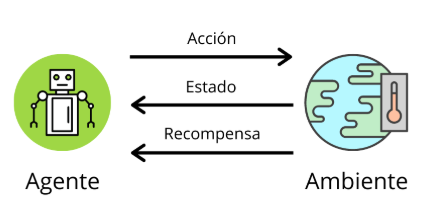
\includegraphics[width=7cm]{figs/introducción/RL.png}
  \end{center}
  \caption{Esquema del proceso de aprendizaje por refuerzo.}
  \label{rl}
\end{figure}

Cada uno de estos enfoques de \ac{ML} tiene sus propias fortalezas y limitaciones. Sin embargo, en la mayoría de los sistemas autónomos modernos, se combinan varias técnicas para garantizar que el vehículo pueda adaptarse a una amplia variedad de condiciones de tráfico y entorno. Al integrar estas soluciones, los coches autónomos pueden mejorar continuamente su rendimiento y fiabilidad.

Este \ac{TFG} propone una solución que combina el aprendizaje supervisado, concretamente redes neuronales para la detección de objetos y de carriles, con el aprendizaje por refuerzo para el control del vehículo. A partir de las observaciones, como los datos de los sensores, y mediante recompensas, el coche aprende a seleccionar las mejores acciones en cada momento.
